% ---------------------------------------------------------------------------------------------
% JustBetter MCP -- token-efficiency benchmark report
%
% Compiles as-is on Overleaf with pdfLaTeX. Every figure is drawn natively with pgfplots, so
% there are no images to upload. Numbers come from benchmark/results/2026-09-26T13-49-49-254Z/
% and can be regenerated with `node benchmark/charts.mjs`.
%
% Replace the \author line with your own name before circulating.
% ---------------------------------------------------------------------------------------------
\documentclass[11pt,a4paper]{article}

\usepackage[utf8]{inputenc}
\usepackage[T1]{fontenc}
\usepackage[margin=2.4cm]{geometry}
\usepackage{booktabs}
\usepackage{graphicx}
\usepackage{xcolor}
\usepackage{pgfplots}
\usepackage{caption}
\usepackage{enumitem}
\usepackage{microtype}
\usepackage[hidelinks]{hyperref}

\pgfplotsset{compat=1.18}
\usepgfplotslibrary{groupplots}

% Arm colours, matched to the figures in README.md
\definecolor{modeone}{HTML}{1F6FEB}
\definecolor{modetwo}{HTML}{BF8700}
\definecolor{modethree}{HTML}{CF222E}

\pgfplotsset{
  benchbar/.style={
    ybar,
    width=\linewidth,
    height=6.4cm,
    ymin=0,
    axis lines*=left,
    ymajorgrids=true,
    grid style={gray!25},
    tick align=outside,
    xtick=data,
    enlarge x limits=0.22,
    legend style={draw=none, fill=none, font=\small},
    label style={font=\small},
    tick label style={font=\small},
    every node near coord/.append style={font=\scriptsize},
    /pgf/number format/.cd, use comma=false, 1000 sep={,}
  }
}

\title{\textbf{Tool Delivery Strategies for MCP Gateways}\\[0.35em]
\large A Controlled Token-Efficiency Benchmark of Semantic Injection,\\
Reactive Discovery, and an Inject-All Baseline}
\author{JustBetter MCP project}
\date{26 September 2026}

\begin{document}
\maketitle

\begin{abstract}
\noindent
Connecting a language model to Model Context Protocol (MCP) servers conventionally means placing
every tool schema from every connected server into every request. With a handful of servers this is
tens of thousands of tokens re-sent on each turn. This report measures three strategies for avoiding
that cost on eight programmatically verified agentic tasks: \textbf{semantic prompt injection}
(retrieve schemas from the user's prompt before the first model call), \textbf{reactive discovery}
(advertise two primitives and let the model fetch schemas mid-conversation, as in Anthropic's MCP
Tool Search and OpenAI Codex's tool search), and an \textbf{inject-all baseline}. Across 24 runs and
916{,}359 provider-reported tokens, semantic injection was cheapest on every aggregate --- a mean of
27{,}251 tokens per run against 39{,}798 for reactive discovery and 47{,}496 for the baseline --- and
matched reactive discovery on task success (7 of 8) while the baseline trailed at 5 of 8.

The mechanism, however, is not the one the project originally hypothesised. Semantic injection and
reactive discovery cost almost exactly the same \emph{per turn} (4{,}542 against 4{,}752 tokens, a
4.6\% gap), and reactive discovery's completion tokens per turn are marginally \emph{lower}, not
higher. Because roughly 97\% of all cost is prompt tokens re-sent each turn, the advantage is
structural: injection reaches the answer in 29\% fewer turns. We also report two genuine defects in
the gateway's tool-retention logic, uncovered by interrogating why an arm was expensive rather than
accepting its number; fixing them reduced cost on two individual tasks by 86\% and 92\%, which is a
larger effect than the difference between any two strategies. Finally, we report a within-arm cost
spread of 4--7$\times$ under greedy decoding, and conclude that at one repetition per cell the
between-arm ordering is directional rather than statistically significant.
\end{abstract}

\vspace{0.4em}
\noindent\textbf{Artefacts.} Task suite and verifiers: \texttt{benchmark/tasks.ts}. Harness:
\texttt{benchmark/run.ts}. Design notes: \texttt{BENCHMARK.md}. Raw per-run records:
\texttt{benchmark/results/2026-09-26T13-49-49-254Z/raw.jsonl}. Figure generator:
\texttt{benchmark/charts.mjs}.

\section{The problem}

An MCP client discovers a server's tools by calling \texttt{tools/list} and then includes those
schemas in the request it sends to the model. The protocol offers no mechanism for partial
disclosure, so the conventional arrangement is all-or-nothing: connect five servers and every
request carries all five servers' schemas, whether the task needs a file reader or a web search.

Three costs follow. The first is direct: schemas occupy prompt tokens, and because an agentic loop
re-sends its entire transcript on every turn, that cost is paid once per turn rather than once per
session. The second is capacity: schemas displace transcript, so a long task hits the context limit
sooner. The third, and least visible, is selection accuracy --- a model choosing among 26 tools
makes different mistakes than one choosing among 5.

A gateway can intercept this. JustBetter MCP sits between the client and the upstream servers,
indexes every tool's name, description, and parameter schema into a vector store, and discloses only
what a turn plausibly needs. The question this report addresses is what that is actually worth, and
by what mechanism.

\section{The three strategies}

All three arms share one agentic loop, one model, one decoding configuration, one task set, and one
verifier per task. They differ only in where the tool array for each request comes from.

\begin{description}[leftmargin=1.4em, itemsep=0.45em]
  \item[Mode 1 --- semantic injection.] The harness posts to the gateway's OpenAI-compatible HTTP
  proxy and sends \emph{no} tools of its own. The proxy embeds the incoming conversation, retrieves
  the top 5 semantic matches from the catalog, adds up to 8 carried-over tools from earlier turns
  plus two fixed fallbacks, and forwards the enriched request upstream. The model never learns this
  happened.

  \item[Mode 2 --- reactive discovery.] The harness posts straight to the provider and supplies the
  tools the gateway advertises over stdio, \textbf{re-listed on every turn}, which is what a
  conformant MCP client does after a \texttt{notifications/tools/list\_changed}. The gateway
  initially advertises only \texttt{request\_tools} and \texttt{batch\_call}; the model must ask for
  what it needs, and matched schemas are both returned in the call result and added to the
  advertised list. This is the strategy Anthropic's MCP Tool Search and OpenAI Codex's tool search
  implement.

  \item[Mode 3 --- inject-all baseline.] Every tool in the catalog, every turn, no retrieval. This is
  what a client does today with no gateway in the path.
\end{description}

\section{Method}

\subsection{Configuration}

\begin{table}[h]
\centering
\small
\begin{tabular}{@{}ll@{}}
\toprule
\textbf{Parameter} & \textbf{Value} \\
\midrule
Model & \texttt{nemotron-3-super} (Ollama Cloud, OpenAI-compatible endpoint) \\
Decoding & \texttt{temperature: 0}, \texttt{reasoning\_effort: low}, no seed \\
Catalog & 26 tools: \texttt{filesystem} + \texttt{terminal} + \texttt{memory} \\
Turn cap & 20 per task (no run reached it) \\
Tasks & 8, each with a programmatic verifier \\
Repetitions & 1 per cell \\
Total runs & 24 (8 tasks $\times$ 3 arms) \\
Tokens consumed & 916{,}359, provider-reported \\
\bottomrule
\end{tabular}
\caption{Experimental configuration.}
\end{table}

Each run gets a freshly created workspace and, for Mode 1 and Mode 2, a freshly spawned gateway
carrying a unique instance token that the harness verifies over the health endpoint before sending
anything. This check exists because an earlier iteration silently reused a stale gateway left
running from a previous session, which invalidated its results.

\subsection{Metrics}

Token counts are the provider's own \texttt{usage} object, read from the response the harness
received, identically for all three arms. No token is estimated or inferred. We report:

\begin{itemize}[leftmargin=1.4em, itemsep=0.2em]
  \item \textbf{Tokens per run} --- mean and median, split into prompt and completion.
  \item \textbf{Tokens per turn} --- total tokens divided by total turns, aggregated per arm. This is
  the stable comparison, because tokens per run is dominated by how many turns a run happened to
  need.
  \item \textbf{Turns per run} --- one turn is one request to the provider.
  \item \textbf{Task success} --- the verifier's verdict, described below.
  \item \textbf{Schemas carried versus schemas called} --- how much of the disclosed tool surface was
  wasted.
\end{itemize}

\subsection{Verification}

Every task ships a verifier that inspects the workspace after the run and returns pass or fail
programmatically. No model is asked for an opinion anywhere. A model judge would consume the same
quota that is under measurement and would inject a second model's variance into the thing being
measured.

Six tasks are verified by their filesystem effect: a file must exist and contain a specific number
or a specific sorted list. One task (\texttt{t7}) has no correct tool --- it asks for an email to be
sent, and no email tool exists in the catalog --- so it is verified on the transcript: claiming
success is a failure, reporting the missing capability is a pass. One task (\texttt{t8}) is
deliberately ambiguous and is verified on two conditions: data must survive, and the model should
seek clarification.

\subsection{Fault classification}

A strict rule separates model failure from everything else: \emph{infrastructure and provider faults
are never scored against a strategy.} Rate limits, transport errors, quota exhaustion, and harness
bugs raise typed exceptions, and the affected run is retried with backoff or abandoned and excluded
rather than recorded as a loss. This matters because the provider imposes one concurrent request and
an unpublished monthly quota, so a badly timed 429 would otherwise look like a strategy that cannot
finish a task.

In the reported run, \textbf{0 runs were abandoned and 0 were retried}. Every failure in
Section~\ref{sec:failures} is the model failing the task.

\section{Results}

\subsection{Headline}

\begin{table}[h]
\centering
\small
\begin{tabular}{@{}lrrrrr@{}}
\toprule
\textbf{Arm} & \textbf{Mean tok/run} & \textbf{Median} & \textbf{Tok/turn} & \textbf{Turns/run} & \textbf{Passed} \\
\midrule
\textbf{Mode 1} --- semantic injection & \textbf{27,251} & \textbf{21,977} & \textbf{4,542} & \textbf{6.0} & 7/8 \\
Mode 2 --- reactive discovery          & 39,798 & 25,255 & 4,752 & 8.4 & 7/8 \\
Mode 3 --- inject-all baseline         & 47,496 & 35,494 & 6,129 & 7.8 & 5/8 \\
\bottomrule
\end{tabular}
\caption{Per-arm aggregates over eight tasks, one run each.}
\label{tab:headline}
\end{table}

Semantic injection is cheapest on every aggregate: 32\% below reactive discovery and 43\% below the
baseline by mean, or 13\% and 38\% by median. The baseline is both the most expensive per turn and
the least reliable. Section~\ref{sec:variance} argues that the median is the figure to quote and that
the ordering should be read as directional.

\begin{figure}[h]
\centering
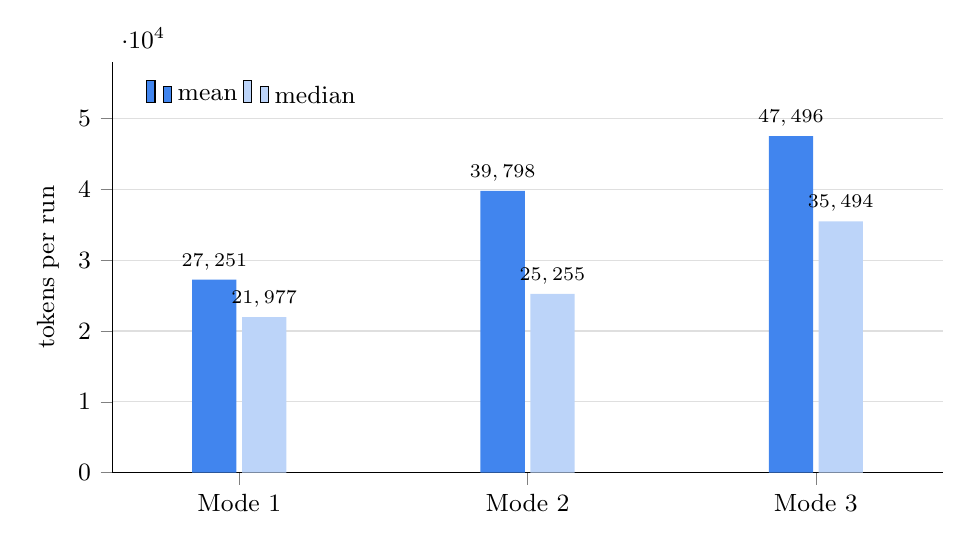
\begin{tikzpicture}
\begin{axis}[
  benchbar,
  ybar,
  bar width=16pt,
  height=6.8cm,
  ylabel={tokens per run},
  symbolic x coords={Mode 1, Mode 2, Mode 3},
  nodes near coords,
  ymax=58000,
  legend pos=north west,
  legend columns=2
]
\addplot[fill=modeone!85, draw=none] coordinates {(Mode 1,27251) (Mode 2,39798) (Mode 3,47496)};
\addplot[fill=modeone!30, draw=none] coordinates {(Mode 1,21977) (Mode 2,25255) (Mode 3,35494)};
\legend{mean, median}
\end{axis}
\end{tikzpicture}
\caption{Mean and median tokens per completed run. The gap between the two within each arm is the
signature of the variance discussed in Section~\ref{sec:variance}: one unlucky run drags the mean
well above the typical case.}
\label{fig:headline}
\end{figure}

\subsection{The mechanism is turn count, not cheaper turns}

The project's stated hypothesis was that pre-injecting schemas spares the model from reasoning about
which tool to fetch, and that this would show up as reduced completion cost. It does not.

\begin{figure}[h]
\centering
\begin{tikzpicture}
\begin{groupplot}[
  group style={group size=2 by 1, horizontal sep=1.9cm},
  benchbar,
  width=0.46\linewidth,
  bar width=15pt,
  symbolic x coords={Mode 1, Mode 2, Mode 3},
  nodes near coords
]
\nextgroupplot[ylabel={tokens per turn}, ymax=7200, title={\small Price of one turn}]
\addplot[ybar, bar shift=0pt, fill=modeone!85, draw=none] coordinates {(Mode 1,4542)};
\addplot[ybar, bar shift=0pt, fill=modetwo!85, draw=none] coordinates {(Mode 2,4752)};
\addplot[ybar, bar shift=0pt, fill=modethree!85, draw=none] coordinates {(Mode 3,6129)};

\nextgroupplot[ylabel={turns per run (mean)}, ymax=10, title={\small Number of turns}]
\addplot[ybar, bar shift=0pt, fill=modeone!85, draw=none] coordinates {(Mode 1,6.0)};
\addplot[ybar, bar shift=0pt, fill=modetwo!85, draw=none] coordinates {(Mode 2,8.4)};
\addplot[ybar, bar shift=0pt, fill=modethree!85, draw=none] coordinates {(Mode 3,7.8)};
\end{groupplot}
\end{tikzpicture}
\caption{Mode 1 and Mode 2 pay nearly the same price per turn --- 4.6\% apart. The entire difference
between them is how many turns they need. Mode 3 is the only arm whose per-turn price is genuinely
higher, because it carries all 26 schemas every time.}
\label{fig:mechanism}
\end{figure}

Table~\ref{tab:split} shows why turn count is decisive. Cost is 97\% prompt in every arm. Completion
is a rounding error. Anything that re-sends the transcript and the tool surface therefore dominates,
and the only lever of consequence is how many times that happens.

\begin{table}[h]
\centering
\small
\begin{tabular}{@{}lrrrrr@{}}
\toprule
\textbf{Arm} & \textbf{Prompt/run} & \textbf{Completion/run} & \textbf{Completion share} & \textbf{Prompt/turn} & \textbf{Completion/turn} \\
\midrule
Mode 1 & 26,484 & 767   & 2.8\% & 4,414 & 128 \\
Mode 2 & 38,812 & 986   & 2.5\% & 4,634 & 118 \\
Mode 3 & 46,013 & 1,483 & 3.1\% & 5,937 & 191 \\
\bottomrule
\end{tabular}
\caption{Where the tokens go. Reasoning tokens are included in completion and pinned to the same
effort level for every arm.}
\label{tab:split}
\end{table}

\paragraph{A retracted claim.} An earlier draft of this work reported that reactive discovery spent
roughly twice semantic injection's completion tokens deliberating over which tool to fetch. That
claim was an artefact of a harness defect (Section~\ref{sec:harnessbug}) and \textbf{does not survive
its correction}. Per turn, reactive discovery's completion cost is marginally \emph{lower} --- 118
against 128. The cost of reactive discovery is extra turns, not extra thinking within a turn. We
report this explicitly because the original claim was the more flattering one for the approach this
project advocates.

\subsection{Tool surface carried, and how much was wasted}

\begin{table}[h]
\centering
\small
\begin{tabular}{@{}lrrr@{}}
\toprule
\textbf{Arm} & \textbf{Schemas per turn} & \textbf{Distinct tools actually called} & \textbf{Never called} \\
\midrule
Mode 1 & 13.2 (mean), 15 (median) & 3 per run (median) & 81\% \\
Mode 2 & not recorded per turn    & 4 per run (median) & --- \\
Mode 3 & 19.9 (mean), 26 (max)    & 3 per run (median) & 88\% \\
\bottomrule
\end{tabular}
\caption{Disclosed surface against used surface. Mode 2's advertised set is not recorded per turn in
this run's raw output, so its waste figure is omitted rather than estimated; structurally, its
unused surface manifests as extra discovery turns instead of carried schemas.}
\label{tab:waste}
\end{table}

Every arm discloses far more than it uses. Retrieval is doing real work --- 13 schemas against the
baseline's 20 --- but a top-5 match plus an 8-slot carry-over is still roughly five times what any of
these tasks needed. \textbf{Retrieval breadth was deliberately not tuned for this run}, so that the
measurement describes the shipped configuration rather than one selected to produce a favourable
result. It is the clearest remaining optimisation target.

One measurement artefact should be noted: the gateway indexes its catalog asynchronously at startup,
so the first turn or two of every run carries only the fallback tools. This affects all arms equally
and should be waited out in future runs.

\subsection{Per-task results}

\begin{table}[h]
\centering
\small
\begin{tabular}{@{}lrrr@{}}
\toprule
\textbf{Task} & \textbf{Mode 1} & \textbf{Mode 2} & \textbf{Mode 3} \\
\midrule
\texttt{t1-read-count}            & 65,539 P & 15,663 P & 35,264 P \\
\texttt{t2-file-size-distractors} & 14,683 P & 20,738 P & 25,466 P \\
\texttt{t3-csv-sum}               & 13,995 P & 20,653 P & 94,026 \textbf{F} \\
\texttt{t4-manifest}              & 25,033 P & 20,626 P & 35,724 P \\
\texttt{t5-newest-file}           & 39,966 P & 29,772 P & 86,714 P \\
\texttt{t6-recover-missing}       &  9,204 P & 31,325 P & 23,544 P \\
\texttt{t7-absent-capability}     & 30,666 P & 75,080 P & 33,526 \textbf{F} \\
\texttt{t8-ambiguous}             & 18,921 \textbf{F} & 104,525 \textbf{F} & 45,706 \textbf{F} \\
\bottomrule
\end{tabular}
\caption{Tokens per task. P denotes a passed verification, \textbf{F} a failed one.}
\label{tab:pertask}
\end{table}

\begin{figure}[h]
\centering
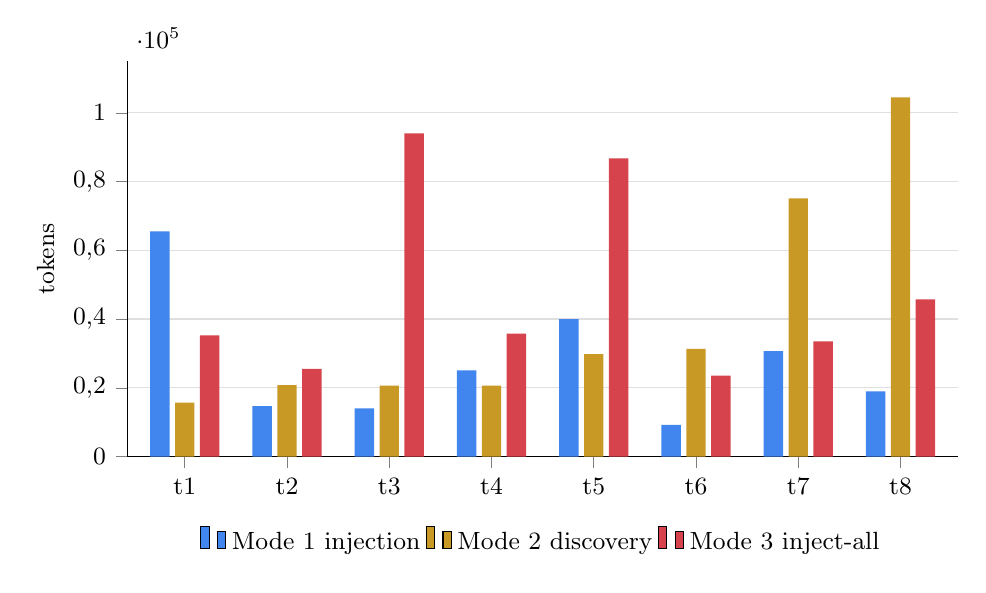
\begin{tikzpicture}
\begin{axis}[
  benchbar,
  bar width=7pt,
  height=6.6cm,
  width=\linewidth,
  ylabel={tokens},
  symbolic x coords={t1,t2,t3,t4,t5,t6,t7,t8},
  enlarge x limits=0.08,
  x tick label style={font=\small},
  legend style={at={(0.5,-0.16)}, anchor=north, legend columns=3}
]
\addplot[fill=modeone!85, draw=none] coordinates {(t1,65539) (t2,14683) (t3,13995) (t4,25033) (t5,39966) (t6,9204) (t7,30666) (t8,18921)};
\addplot[fill=modetwo!85, draw=none] coordinates {(t1,15663) (t2,20738) (t3,20653) (t4,20626) (t5,29772) (t6,31325) (t7,75080) (t8,104525)};
\addplot[fill=modethree!85, draw=none] coordinates {(t1,35264) (t2,25466) (t3,94026) (t4,35724) (t5,86714) (t6,23544) (t7,33526) (t8,45706)};
\legend{Mode 1 injection, Mode 2 discovery, Mode 3 inject-all}
\end{axis}
\end{tikzpicture}
\caption{Per-task cost. The ordering is not uniform: reactive discovery wins three of the eight tasks
outright. The range within a single arm is as large as the difference between arms, which is the
substance of Section~\ref{sec:variance}.}
\label{fig:pertask}
\end{figure}

\section{Defects found, and what fixing them was worth}
\label{sec:defects}

Two genuine defects in the gateway were found during this work, both by asking \emph{why} an arm was
expensive rather than accepting its number. Each is a defect in the gateway rather than in the
benchmark, and each now carries a regression test.

\subsection{Retention was ordered alphabetically, not by recency}

The query selecting which tools to carry into the next turn read
\texttt{ORDER BY injected\_at DESC, tool\_name ASC}. But \texttt{injected\_at} is populated from
SQLite's \texttt{CURRENT\_TIMESTAMP}, which resolves only to the second, so every tool injected
during one turn carried an identical timestamp. The recency sort was a no-op, and the effective
ordering was its tiebreak: \textbf{alphabetical by tool name}.

Among the filesystem tools, \texttt{write\_file} sorts last. It could therefore never survive an
eight-slot window. On any task that reads and then writes, the model discovered \texttt{write\_file},
lost it, and rediscovered it --- measured at ten consecutive \texttt{request\_tools} calls on a single
task. The fix is a monotonic per-injection sequence counter, so the ordering is the recency the query
had always claimed.

\subsection{The model's own discoveries were outranked by routine injections}

The same retention pool received two very different kinds of entry with equal standing: the fifteen
or more tools the gateway injected speculatively each turn, and the tools the model had explicitly
asked for through \texttt{request\_tools}. The speculative majority evicted the deliberate minority.
The code comment described the pool as holding ``recently \emph{requested}'' tools; nothing tracked
requests at all.

The fix marks requested tools with a flag that outranks routine injections, sticky for the remainder
of the session so that a later speculative injection cannot silently demote them.

\subsection{Measured effect}

\begin{table}[h]
\centering
\small
\begin{tabular}{@{}lrrr@{}}
\toprule
\textbf{Task} & \textbf{Before} & \textbf{After} & \textbf{Change} \\
\midrule
\texttt{t1-read-count}            & 76,305 / 10 turns & 10,788 / 4 turns & $-$86\% \\
\texttt{t2-file-size-distractors} & 149,892 / 15 turns & 11,382 / 4 turns & $\mathbf{-92\%}$ \\
\bottomrule
\end{tabular}
\caption{Same task, same model, same decoding, before and after the two retention fixes.}
\label{tab:fixes}
\end{table}

\textbf{These fixes were worth considerably more than the difference between any two strategies.}
Before them, semantic injection measured as the \emph{most} expensive arm; after them it is the
cheapest. Any published comparison of tool-delivery strategies is, to a substantial degree, a
comparison of implementation quality --- a caveat that applies to this report as much as to any
other.

\subsection{A third fix, in the prompt}

The tool-access section of the injected system prompt unconditionally asserted that the capabilities
listed below were not yet loaded and that the model must call \texttt{request\_tools} to obtain them
--- followed by the list of tools \emph{not} injected that turn. When that list is empty, which is
always true under inject-all and true under semantic injection whenever retrieval covers the
catalog, the instruction is simply false. The model obeyed it regardless: one \texttt{list\_directory}
followed by nine \texttt{request\_tools} calls, 78{,}765 tokens, task failed. The instruction is now
issued only when something is genuinely undisclosed; on that task the cost fell to 33{,}205 tokens
and it passed.

\subsection{A harness defect, for completeness}
\label{sec:harnessbug}

The harness originally called \texttt{listTools()} once, outside the agentic loop, so Mode 2 carried
two schemas per turn while Mode 1 carried fifteen. This understated Mode 2's cost by roughly half and
would have produced a false result \emph{in favour of the approach this project advocates}, since the
inflated completion-token gap was read as evidence for the deliberation hypothesis. It was caught by
noticing that a per-turn schema count of two was inconsistent with a conformant client's behaviour.
The harness now re-lists on every turn.

\section{Variance, and why single runs cannot settle this}
\label{sec:variance}

\begin{table}[h]
\centering
\small
\begin{tabular}{@{}lrrrr@{}}
\toprule
\textbf{Arm} & \textbf{Min} & \textbf{Median} & \textbf{Max} & \textbf{Spread} \\
\midrule
Mode 1 &  9,204 & 21,977 &  65,539 & 7.1$\times$ \\
Mode 2 & 15,663 & 25,255 & 104,525 & 6.7$\times$ \\
Mode 3 & 23,544 & 35,494 &  94,026 & 4.0$\times$ \\
\bottomrule
\end{tabular}
\caption{Within-arm cost range across the eight tasks.}
\label{tab:variance}
\end{table}

Some of that range is task difficulty. Some is not. Task \texttt{t1-read-count} under semantic
injection cost \textbf{10{,}788 tokens in 4 turns} on one execution and \textbf{65{,}539 in 10} on
another, with identical code, identical inputs, and \texttt{temperature: 0}. The model emits reasoning
and no seed was set, so runs are not reproducible even under greedy decoding.

\textbf{Consequence: the ordering in Table~\ref{tab:headline} is directional, not significant.} One
repetition per cell cannot separate a 13\% median difference from noise of this magnitude. Readers
quoting these results should quote the medians, the spread, and this paragraph together.

\section{Failures, examined individually}
\label{sec:failures}

Because no run was abandoned or retried, every failure below is the model failing the task rather
than an infrastructure fault.

\begin{description}[leftmargin=1.4em, itemsep=0.5em]
  \item[\texttt{t3-csv-sum}, Mode 3 (94{,}026 tokens, 11 turns).] Called \texttt{request\_tools} eight
  times despite being told explicitly that every tool was already present in its array and that it
  should not. The description of \texttt{batch\_call} does itself mention ``any tool name returned by
  \texttt{request\_tools}'', which may nudge the model in that direction, but this is model behaviour
  against an explicit instruction rather than a prompt defect.

  \item[\texttt{t7-absent-capability}, Mode 3.] Claimed the email had been sent. No email tool exists
  anywhere in the catalog. This is precisely the failure mode the task exists to detect, and only the
  inject-all baseline fell for it --- weak evidence that a large undifferentiated tool surface makes
  a model likelier to believe it has a capability it lacks.

  \item[\texttt{t8-ambiguous}, all three arms.] The prompt is ``Clean up my working folder'', for which
  the correct behaviour is to ask what that means. \textbf{No arm asked.} Equally, no arm destroyed
  data: the file marked as important survived in all three. Reactive discovery spent 104{,}525 tokens
  and 17 turns, including eight consecutive \texttt{search\_files} calls, exploring rather than asking.

  The verifier for this task requires a literal question mark in the assistant's text, which is a
  crude operationalisation of ``sought clarification''. This row should be read as \emph{no arm sought
  clarification and no arm destroyed data} rather than as a clean three-way failure.
\end{description}

\section{Threats to validity}

\begin{itemize}[leftmargin=1.4em, itemsep=0.3em]
  \item \textbf{One repetition per cell.} See Section~\ref{sec:variance}. This is the dominant
  limitation of the study.
  \item \textbf{One model.} A result on \texttt{nemotron-3-super} is a result about that model. A
  second model was considered and dropped because its free tier was too rate-limited for clean runs.
  \item \textbf{Eight tasks}, all filesystem-and-shell shaped, written by the same person holding the
  hypothesis. The suite and its verifiers are published so that these choices can be disputed.
  \item \textbf{Tokens, not money.} Prompt caching was left enabled but unmeasured. The inject-all
  baseline has the most static prefix and will cache best, so its real monetary cost is lower than
  its token count implies. Nothing here is a cost claim.
  \item \textbf{Reasoning tokens} are included in completion and pinned to the same effort level for
  every arm, so these totals do not transfer to a non-reasoning model.
  \item \textbf{Mode 2's harness is not Claude Desktop or Cursor.} Those products bring their own
  system prompts and loops. This measures the strategy, not those implementations.
  \item \textbf{Asynchronous catalog indexing} leaves the first turn or two of every run
  under-provisioned. This affects all arms equally but should be waited out.
  \item \textbf{Retrieval breadth was not tuned.} Semantic injection carries roughly 15 schemas to
  call 3. Both widening and narrowing were left alone deliberately, so this measures the shipped
  configuration.
  \item \textbf{Implementation quality is confounded with strategy.} Section~\ref{sec:defects}
  demonstrates that two ordinary bugs moved individual task costs by 86--92\%, far more than the
  between-strategy differences reported here.
\end{itemize}

\section{What would strengthen this}

In order of value per token spent:

\begin{enumerate}[leftmargin=1.6em, itemsep=0.3em]
  \item \textbf{Three repetitions per cell}, which would turn Table~\ref{tab:headline} from
  directional into arguable. This is the only change that addresses the dominant limitation.
  \item \textbf{Catalog scaling.} One task across catalogs of roughly 10, 25, 50, and 100 tools,
  reporting tokens per additional tool. A slope predicts catalog sizes nobody has tested, which is
  what the premise of a gateway most needs.
  \item \textbf{A fixed seed}, to separate model nondeterminism from real effects.
  \item \textbf{Tuning retrieval breadth} now that the retention defects are fixed, given that 81\%
  of carried schemas were never called.
  \item \textbf{A second model}, to establish whether the turn-count mechanism generalises.
\end{enumerate}

\section{Reproducing}

\begin{verbatim}
node benchmark/catalog.mjs        # measure the tool catalog; costs no provider tokens
npx tsx benchmark/run.ts          # the full suite
node benchmark/status.mjs         # progress and interim results, safe to run mid-suite
node benchmark/charts.mjs         # redraw the figures from raw.jsonl
BENCH_RESUME=<dir> npx tsx benchmark/run.ts    # continue an interrupted suite
\end{verbatim}

\noindent
Environment overrides: \texttt{BENCH\_MODEL}, \texttt{BENCH\_BAND}
(\texttt{small}/\texttt{medium}/\texttt{large}), \texttt{BENCH\_TASKS} (comma-separated),
\texttt{BENCH\_BUDGET\_TOKENS}, \texttt{BENCH\_BUDGET\_MINUTES}, \texttt{BENCH\_REASONING}.

\begin{thebibliography}{9}
\bibitem{mcp} Anthropic. \emph{Model Context Protocol specification}.
\url{https://modelcontextprotocol.io}
\bibitem{repo} \emph{JustBetter MCP}. \url{https://www.npmjs.com/package/justbetter-mcp}
\bibitem{sqlitevec} A. Lee. \emph{sqlite-vec: a vector search extension for SQLite}.
\url{https://github.com/asg017/sqlite-vec}
\end{thebibliography}

\end{document}
